% lecture07.tex — Morse Functions

\section{Morse Functions}

Consider a smooth function $f \colon M \to \R$. If $x \in M$ is a regular point of $f$ (i.e.\ if $df_x \neq 0$), we know that we can choose a local coordinate around $x$ so that $f$ is simply the first coordinate function.

What can we say at critical points?

Recall from calculus that a critical point $x$ of $f \colon \R^k \to \R$ is called \emph{nondegenerate} if the \emph{Hessian matrix} $H = \left(\frac{\partial^2 f}{\partial x_i \partial x_j}\right)$ is nonsingular at $x$.

\begin{center}
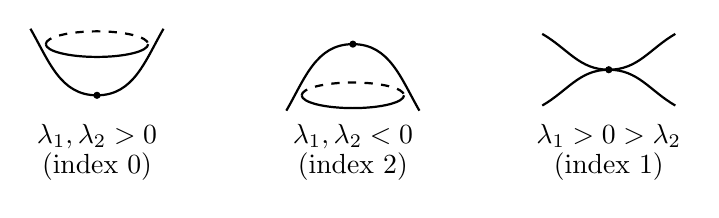
\begin{tikzpicture}[scale=0.65]
    % Index 0: bowl up
    \draw[thick] (-1.3,1.8) to[out=-60,in=180] (0,0.5) to[out=0,in=240] (1.3,1.8);
    \draw[thick] (-1,1.5) arc(180:360:1 and 0.25);
    \draw[thick,dashed] (-1,1.5) arc(180:0:1 and 0.25);
    \fill (0,0.5) circle (2pt);
    \node at (0,-0.3) {$\lambda_1, \lambda_2 > 0$};
    \node at (0,-0.9) {(index $0$)};
    % Index 2: bowl down
    \begin{scope}[xshift=5cm]
        \draw[thick] (-1.3,0.2) to[out=60,in=180] (0,1.5) to[out=0,in=120] (1.3,0.2);
        \draw[thick] (-1,0.5) arc(180:360:1 and 0.25);
        \draw[thick,dashed] (-1,0.5) arc(180:0:1 and 0.25);
        \fill (0,1.5) circle (2pt);
        \node at (0,-0.3) {$\lambda_1, \lambda_2 < 0$};
        \node at (0,-0.9) {(index $2$)};
    \end{scope}
    % Index 1: saddle
    \begin{scope}[xshift=10cm]
        \draw[thick] (-1.3,0.3) to[out=30,in=180] (0,1) to[out=0,in=150] (1.3,0.3);
        \draw[thick] (-1.3,1.7) to[out=-30,in=180] (0,1) to[out=0,in=210] (1.3,1.7);
        \fill (0,1) circle (2pt);
        \node at (0,-0.3) {$\lambda_1 > 0 > \lambda_2$};
        \node at (0,-0.9) {(index $1$)};
    \end{scope}
\end{tikzpicture}
\end{center}

\begin{proposition}{Nondegenerate Critical Points are Isolated}{nondeg-isolated}
    Nondegenerate critical points are isolated from the other critical points.
\end{proposition}

\begin{proof}
    Consider the map $\nabla f \colon \R^k \to \R^k$, $x \mapsto \left(\frac{\partial f}{\partial x_1}(x), \ldots, \frac{\partial f}{\partial x_k}(x)\right)$. Then $\nabla f(x) = 0$, since $x$ is a critical point. Nondegeneracy means $d(\nabla f)_x$ is a local diffeomorphism at $x$. Thus $f$ has no other critical point in a small neighborhood of $x$.
\end{proof}

\subsection{Nondegeneracy on Manifolds}

Nondegeneracy of critical points makes sense on manifolds, thanks to the following:

\begin{lemma}{Nondegeneracy is Independent of Coordinates}{nondeg-coords}
    Suppose $f \colon \R^k \to \R$ has a nondegenerate critical point at $0$ and $\psi$ is a diffeomorphism with $\psi(0) = 0$. Then $f \circ \psi$ also has a nondegenerate critical point at $0$.
\end{lemma}

\begin{proof}
    Let $f' = f \circ \psi$. Then
    \[
        \frac{\partial f'}{\partial x_i}(x) = \sum_\alpha \frac{\partial f}{\partial x_\alpha}(\psi(x)) \frac{\partial \psi_\alpha}{\partial x_i}(x),
    \]
    and
    \[
        \frac{\partial^2 f'}{\partial x_i \partial x_j}(0) = \sum_\alpha \sum_\beta \frac{\partial^2 f}{\partial x_\alpha \partial x_\beta}(0) \frac{\partial \psi_\alpha}{\partial x_i}(0) \frac{\partial \psi_\beta}{\partial x_j}(0) + \sum_\alpha \frac{\partial f}{\partial x_\alpha}(0) \frac{\partial^2 \psi_\alpha}{\partial x_i \partial x_j}(0).
    \]
    The last sum vanishes since $0$ is a critical point. That is, the new Hessian is $H' = (d\psi_0)^t H (d\psi_0)$. Since $H$ and $d\psi_0$ are nonsingular, so is $H'$.
\end{proof}

\begin{definition}{Morse Function}{morse-function}
    A function $f \colon M \to \R$ whose critical points are all nondegenerate is called a \emph{Morse function}.
\end{definition}

Morse functions are extremely important! They tell us a great deal about the topology of $M$, and much of modern topology is based on this idea. It'll take another whole course to talk about Morse theory, but let me just mention:

\emph{Morse lemma}: If $a \in M$ is a nondegenerate critical point of $f$, then there is a local coordinate system $(x_1, \ldots, x_m)$ around $a$ such that
\[
    f = f(a) + \sum h_{ij} x_i x_j \quad \text{near } a,
\]
i.e.\ $f$ is locally a quadratic polynomial.

\subsection{Abundance of Morse Functions}

As an application of Sard's theorem, let's show that the vast majority of functions are Morse functions.

\begin{theorem}{Generic Functions are Morse}{generic-morse}
    Let $f \colon M \to \R$ be a function, and suppose our manifold $M$ sits inside $\R^N$. For each $a = (a_1, \ldots, a_N) \in \R^N$, define
    \[
        f_a := f + a_1 x_1 + \cdots + a_N x_N,
    \]
    where $x_1, \ldots, x_N$ are the usual coordinate functions on $\R^N$. Then, for almost every $a \in \R^N$, $f_a$ is a Morse function.
\end{theorem}

\begin{proof}
    Let's first prove the result in $\R^k$:

    \begin{lemma}{Local Morse Genericity}{local-morse}
        Let $f \colon U \subset \R^k \to \R$ be a smooth function. Then, for almost all $a = (a_1, \ldots, a_k) \in \R^k$,
        \[
            f_a := f + a_1 x_1 + \cdots + a_k x_k
        \]
        is a Morse function on $U$.
    \end{lemma}

    \begin{proof}
        Note that $(df_a)_p = \left(\frac{\partial f_a}{\partial x_1}(p), \ldots, \frac{\partial f_a}{\partial x_k}(p)\right) = \nabla f(p) + a$, so $p$ is a critical point of $f_a$ iff $\nabla f(p) = -a$. Moreover, it's nondegenerate iff $d(\nabla f)_p$ is nonsingular, i.e.\ if $p$ is a regular point of $\nabla f$.

        Thanks to Sard, $-a$ is a regular value of $\nabla f$ for almost all $a \in \R^k$.
    \end{proof}

    Now let's turn this into a global result. Suppose $p \in M$ and $x_1, \ldots, x_N$ are the standard coordinate functions on $\R^N$. Then, some $m$ of these coordinate functions, $x_{i_1}, \ldots, x_{i_m}$, constitute a coordinate system in a neighborhood of $p$.

    Hence, we can cover $M$ with countably many such open subsets $U_\alpha$, and it suffices to show that $f_a$ is Morse on $U_\alpha$ for almost every $a \in \R^N$.

    For convenience, assume that $(x_1, \ldots, x_m)$ is a coordinate system on $U_\alpha$. Let $S_\alpha = \{a \in \R^N \mid f_a \text{ is not Morse on } U_\alpha\}$.

    Then, by the lemma, $S_\alpha \cap (\R^m \times \{c\})$ has measure zero in $\R^m$, for any $c = (c_{m+1}, \ldots, c_N)$. By Fubini, it follows that $S_\alpha$ has measure zero.
\end{proof}
